%%%%%%%%%%%%%%%%%%%%%%%%%%%%%%%%%%%%%%%%%%%%%%%%%%%%%%%%%%%%%%%%%%%%%%
% Trabalho P2 - Machine Learning (Regressão)
% Predição Salarial na Área de Ciência de Dados
%%%%%%%%%%%%%%%%%%%%%%%%%%%%%%%%%%%%%%%%%%%%%%%%%%%%%%%%%%%%%%%%%%%%%%

\documentclass[12pt]{article}

\usepackage{float}
\usepackage{sbc-template}
\bibliographystyle{sbc}
\usepackage{amsmath}
\usepackage{graphicx,url}

%\usepackage[brazil]{babel}   
\usepackage[utf8]{inputenc}  

     
\sloppy
  
\title{Aplicação de Técnicas de Aprendizado de Máquina para Predição Salarial na Área de Ciência de Dados}

\author{Gustavo X. Saldanha\inst{1}, Lucas Santos\inst{1}, Miguel Bianchini\inst{1} }


\address{Centro Federal de Educação Tecnológica Celso Suckow da Fonseca - Cefet/RJ\\
Campus Nova Friburgo\\
Av. Gov. Roberto Silveira, 1900 - Jardim Ouro Preto, Nova Friburgo - RJ
  \email{\{gustavo.saldanha,lucas.santos,miguel.bianchini\}@aluno.cefet-rj.br}
}

\begin{document} 

\maketitle

\begin{resumo} 
Este trabalho aplica técnicas de aprendizado de máquina supervisionado para a predição salarial de profissionais da área de Ciência de Dados. A base de dados utilizada, ``Data Science Job Salaries'', contém informações sobre nível de experiência, tipo de contratação, cargo, localização e porte da empresa, além do salário anual em dólares. Foram avaliados seis modelos de regressão --- Regressão Linear, Regressão Polinomial, Árvore de Decisão, Random Forest, Support Vector Machines (SVR) e Redes Neurais (MLP) --- com diferentes configurações de pré-processamento. A Árvore de Decisão com profundidade 3 obteve o melhor desempenho ($R^2 = 0{,}514$, $MAE \approx \$37.000$), seguida pela Regressão Linear ($R^2 = 0{,}455$). Os resultados indicam que modelos mais simples apresentam melhor capacidade de generalização para este problema.
\end{resumo}

\section{Introdução}

A área de Ciência de Dados tem apresentado crescimento significativo nos últimos anos, impulsionado pela demanda crescente por soluções baseadas em dados e inteligência artificial. Esse cenário resultou em ampla diversidade de cargos, níveis de experiência e modalidades de trabalho, tornando a análise salarial um tema relevante para profissionais e empresas do setor.

Neste trabalho, foi utilizada a base de dados ``Data Science Job Salaries'' \cite{ds_salary_dataset}, disponibilizada na plataforma Kaggle, contendo informações sobre experiência profissional, tipo de contratação, cargo exercido, localização geográfica, modalidade de trabalho remoto e porte da empresa, além do salário anual convertido para dólares americanos. O objetivo é aplicar técnicas de regressão supervisionada para predição do salário a partir dessas variáveis.

Foram avaliados seis modelos de regressão: Regressão Linear, Regressão Polinomial, Árvore de Decisão, Random Forest, Support Vector Machines (SVR) e Redes Neurais Artificiais (MLP). Cada modelo foi testado em quatro variações de pré-processamento, permitindo analisar o impacto da codificação de variáveis categóricas e da padronização no desempenho preditivo.

A avaliação dos modelos foi realizada por meio de métricas de regressão: coeficiente de determinação ($R^2$), erro absoluto médio (MAE), raiz do erro quadrático médio (RMSE) e erro percentual absoluto médio (MAPE), permitindo uma comparação consistente entre as diferentes abordagens.


\section{Trabalhos Relacionados} \label{sec:related}

A predição salarial é um tema frequentemente abordado na literatura de aprendizado de máquina, especialmente no contexto de análise do mercado de trabalho em tecnologia. Diversos estudos utilizam bases de dados públicas de plataformas como Kaggle para investigar os fatores que influenciam a remuneração de profissionais de dados \cite{ds_salary_dataset}.

Na área de predição numérica, a aplicação de algoritmos de regressão supervisionada é consolidada. Hastie, Tibshirani e Friedman \cite{hastie2009} apresentam os fundamentos teóricos dos métodos de regressão, incluindo modelos lineares, árvores de decisão e Support Vector Machines, discutindo o trade-off entre viés e variância que é central para o problema de predição salarial.

Géron \cite{geron2019} apresenta aplicações práticas de modelos como Random Forest e Redes Neurais para tarefas de regressão, destacando a importância do pré-processamento de dados e da engenharia de atributos no desempenho dos modelos. Smola e Schölkopf \cite{smola2004} detalham o uso de Support Vector Machines para regressão, fundamentando o SVR utilizado neste trabalho.

Dessa forma, a aplicação de técnicas de aprendizado de máquina para análise salarial constitui uma abordagem relevante e consolidada, servindo como base para o desenvolvimento deste trabalho.


\section{Metodologia}

Os experimentos seguiram um fluxo padronizado para todos os modelos:

\begin{enumerate}
    \item \textbf{Pré-processamento:} limpeza dos dados, engenharia de atributos, codificação de variáveis categóricas e divisão treino/teste (75\%/25\%);
    \item \textbf{Geração de variações:} quatro combinações de codificação (One-Hot ou Label Encoding) e padronização (com ou sem StandardScaler);
    \item \textbf{Treinamento:} cada modelo foi avaliado em todas as variações, com diferentes hiperparâmetros;
    \item \textbf{Avaliação:} as métricas $R^2$, MAE, RMSE e MAPE foram calculadas no conjunto de teste;
    \item \textbf{Seleção:} a melhor configuração por modelo foi identificada pelo maior $R^2$ no teste.
\end{enumerate}

Os experimentos foram implementados em Python utilizando Scikit-learn, Pandas e NumPy. O código-fonte está disponível em: \url{https://github.com/lucastak/college-machine-learning}.


\section{Obtenção e preparação dos dados}

\subsection{Descrição do Dataset}

A base de dados ``Data Science Job Salaries'' \cite{ds_salary_dataset} contém 607 registros de salários de profissionais da área de Ciência de Dados. Após remoção de 42 linhas duplicadas, o dataset final possui 565 registros.

A variável alvo é o \textit{salary\_in\_usd} (salário anual em dólares). As colunas \textit{salary} e \textit{salary\_currency} foram removidas para evitar \textit{data leakage}, por serem diretamente derivadas do valor alvo. A Tabela~\ref{tab:variaveis} apresenta as variáveis utilizadas.

\begin{table}[H]
\centering
\caption{Variáveis do dataset}
\label{tab:variaveis}
\begin{tabular}{|l|l|l|}
\hline
\textbf{Variável} & \textbf{Descrição} & \textbf{Tipo} \\ \hline
work\_year & Ano de referência (2020--2022) & Numérica \\ \hline
experience\_level & EN, MI, SE, EX & Categórica ordinal \\ \hline
employment\_type & FT, PT, CT, FL & Categórica nominal \\ \hline
job\_title & Cargo exercido ($\sim$50 categorias) & Categórica nominal \\ \hline
employee\_residence & País de residência & Categórica nominal \\ \hline
remote\_ratio & Percentual remoto (0, 50, 100) & Numérica \\ \hline
company\_location & País da empresa & Categórica nominal \\ \hline
company\_size & S, M, L & Categórica nominal \\ \hline
salary\_in\_usd & Salário anual em USD & Numérica (target) \\ \hline
\end{tabular}
\end{table}

\subsection{Engenharia de Atributos}

Duas novas variáveis foram criadas para melhorar a capacidade preditiva:

\begin{itemize}
    \item \textbf{job\_group}: agrupamento dos $\sim$50 cargos em 6 categorias --- Data Scientist, Data Engineer, ML Engineer, Data Analyst, Manager/Director e Research/AI --- reduzindo a esparsidade;
    \item \textbf{is\_us\_company}: variável binária indicando se a empresa é sediada nos EUA. Essa distinção é relevante pois a mediana salarial de empresas americanas (\$133K) é aproximadamente o dobro de empresas de outros países (\$63K).
\end{itemize}

\subsection{Análise Exploratória}

A Figura~\ref{fig:dist_target} apresenta a distribuição da variável alvo. Observa-se uma distribuição assimétrica positiva, com concentração de salários entre \$50K e \$150K e presença de outliers acima de \$400K.

\begin{figure}[H]
    \centering
    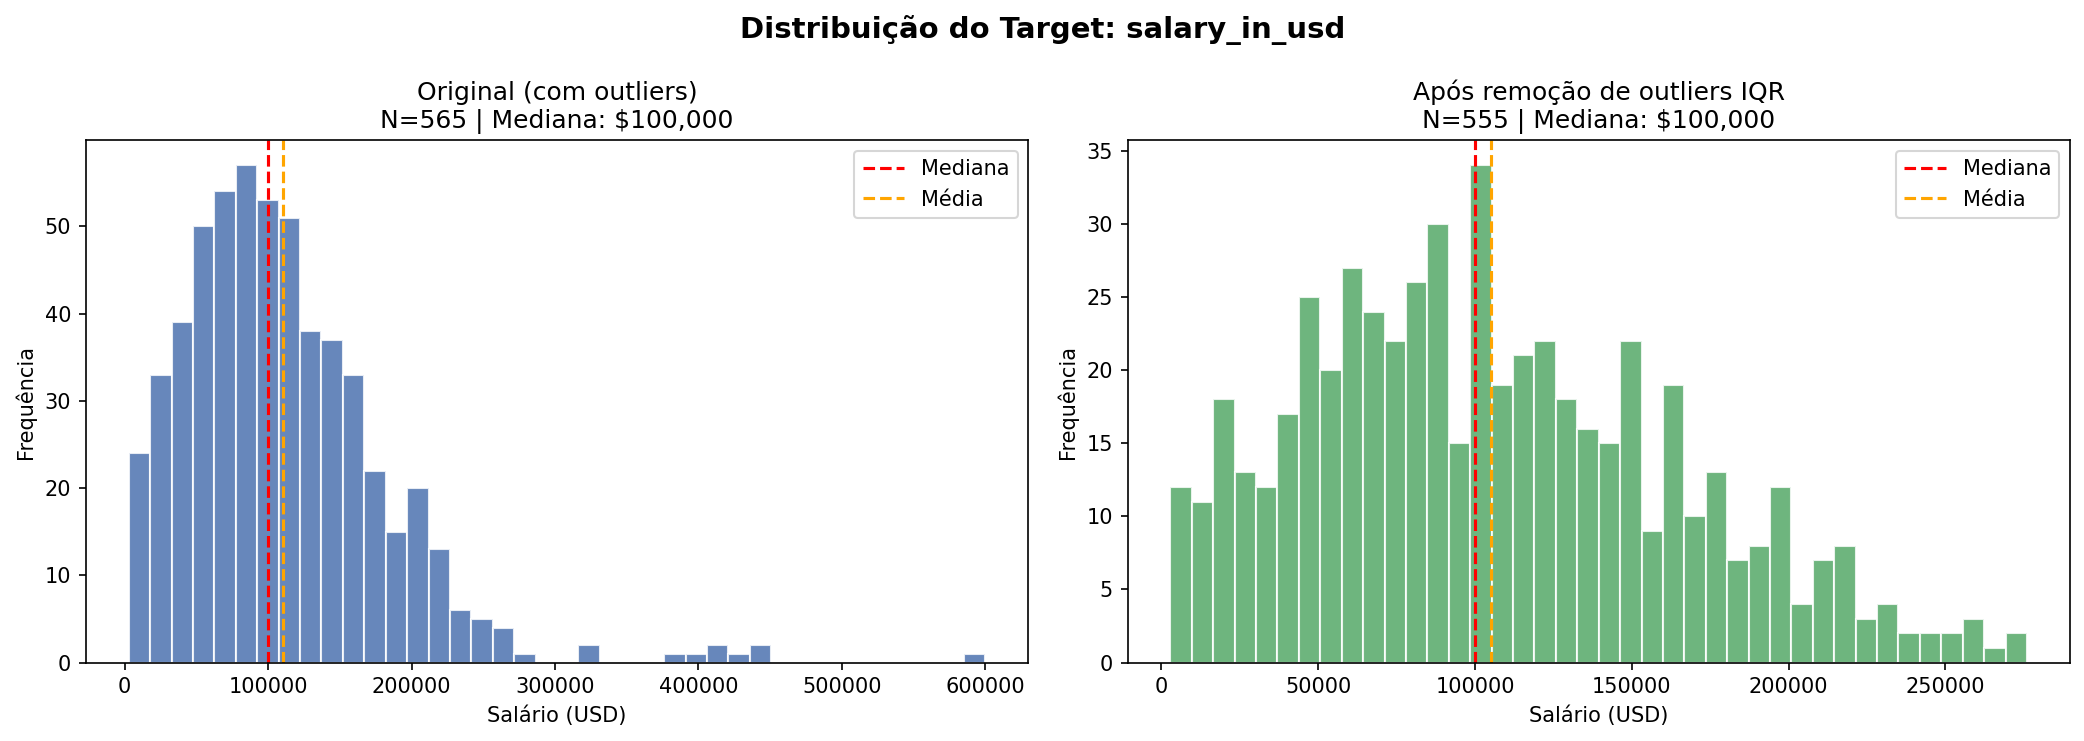
\includegraphics[width=0.85\textwidth]{imagens/eda/01_distribuicao_target.png}
    \caption{Distribuição do salário anual em USD}
    \label{fig:dist_target}
\end{figure}

A Figura~\ref{fig:sal_exp} ilustra a relação entre nível de experiência e salário. Profissionais de nível \textit{Executive} apresentam os maiores salários, seguidos por \textit{Senior}, \textit{Mid-level} e \textit{Entry-level}, confirmando a importância dessa variável para o modelo.

\begin{figure}[H]
    \centering
    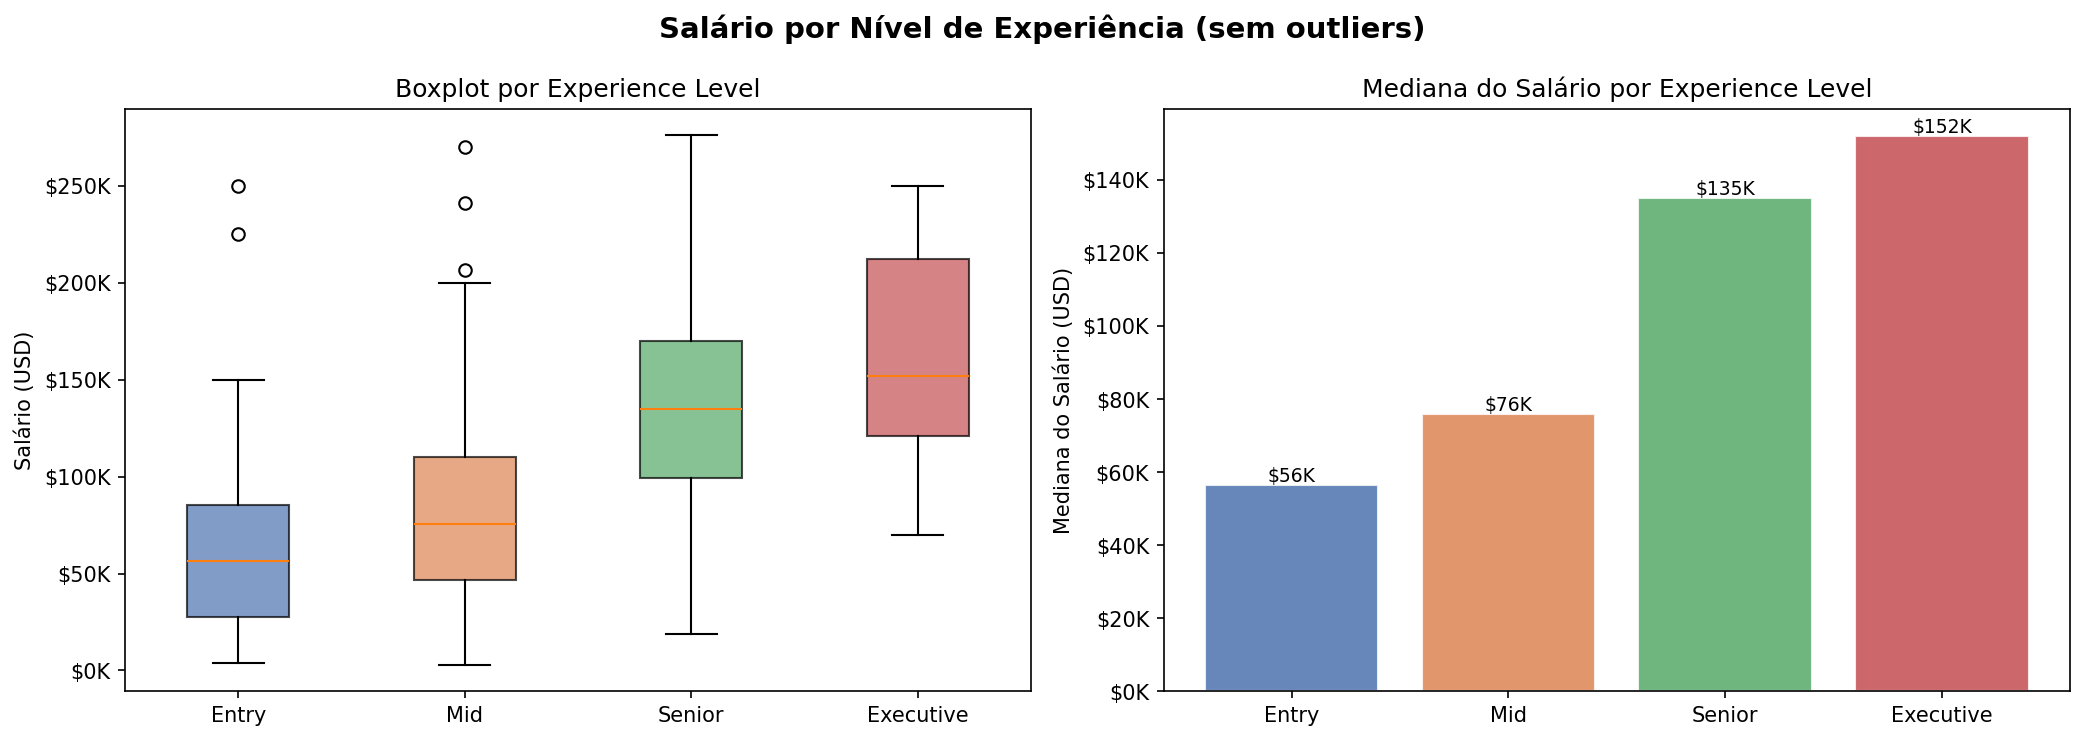
\includegraphics[width=0.85\textwidth]{imagens/eda/03_salario_por_experience.png}
    \caption{Distribuição salarial por nível de experiência}
    \label{fig:sal_exp}
\end{figure}


\subsection{Codificação e Pré-processamento}

A variável \textit{experience\_level} foi codificada com \textit{OrdinalEncoder} (EN=0, MI=1, SE=2, EX=3), preservando sua ordem natural. Para as demais variáveis categóricas, foram testadas duas abordagens:

\begin{itemize}
    \item \textbf{One-Hot Encoding} (\textit{com\_dummy}): expande para 125 atributos, evitando relações ordinais artificiais;
    \item \textbf{Label Encoding} (\textit{sem\_dummy}): mantém 9 atributos, atribuindo inteiros às categorias.
\end{itemize}

Adicionalmente, foi avaliado o impacto da padronização com \textit{StandardScaler}. A combinação dessas opções gerou quatro variações da base, conforme a Tabela~\ref{tab:variacoes}.

\begin{table}[H]
\centering
\caption{Variações de pré-processamento}
\label{tab:variacoes}
\begin{tabular}{|l|l|l|c|}
\hline
\textbf{Variação} & \textbf{Encoding} & \textbf{Padronização} & \textbf{Features} \\ \hline
com\_dummy\_com\_std & One-Hot & StandardScaler & 125 \\ \hline
com\_dummy\_sem\_std & One-Hot & Nenhuma & 125 \\ \hline
sem\_dummy\_com\_std & Label Encoding & StandardScaler & 9 \\ \hline
sem\_dummy\_sem\_std & Label Encoding & Nenhuma & 9 \\ \hline
\end{tabular}
\end{table}

Os dados foram divididos em 75\% para treinamento ($\sim$424 amostras) e 25\% para teste ($\sim$141 amostras), com \texttt{random\_state=0} para reprodutibilidade.


\section{Resultados e Discussões}

Nesta seção são apresentados os resultados obtidos para cada modelo de regressão. A análise foca nas métricas de desempenho e na comparação entre as diferentes configurações de pré-processamento e hiperparâmetros.

\subsection{Regressão Linear}

A Regressão Linear foi avaliada nas quatro variações da base de dados. A Tabela~\ref{tab:lr_resultados} apresenta os resultados obtidos.

\begin{table}[H]
\centering
\caption{Resultados da Regressão Linear por variação de pré-processamento}
\label{tab:lr_resultados}
\begin{tabular}{|l|c|c|c|c|}
\hline
\textbf{Base} & \textbf{$R^2$} & \textbf{MAE (USD)} & \textbf{RMSE (USD)} & \textbf{MAPE (\%)} \\ \hline
com\_dummy\_sem\_std & \textbf{0,4549} & \textbf{39.763} & \textbf{56.109} & \textbf{72,41} \\ \hline
com\_dummy\_com\_std & 0,4533 & 39.708 & 56.190 & 72,30 \\ \hline
sem\_dummy\_com\_std & 0,4274 & 39.862 & 57.506 & 84,20 \\ \hline
sem\_dummy\_sem\_std & 0,4274 & 39.862 & 57.506 & 84,20 \\ \hline
\end{tabular}
\end{table}

A melhor configuração utilizou a base \textit{com\_dummy\_sem\_std} (One-Hot Encoding sem padronização), obtendo $R^2 = 0{,}4549$, $MAE \approx \$39.763$ e $RMSE \approx \$56.109$.

\begin{figure}[H]
    \centering
    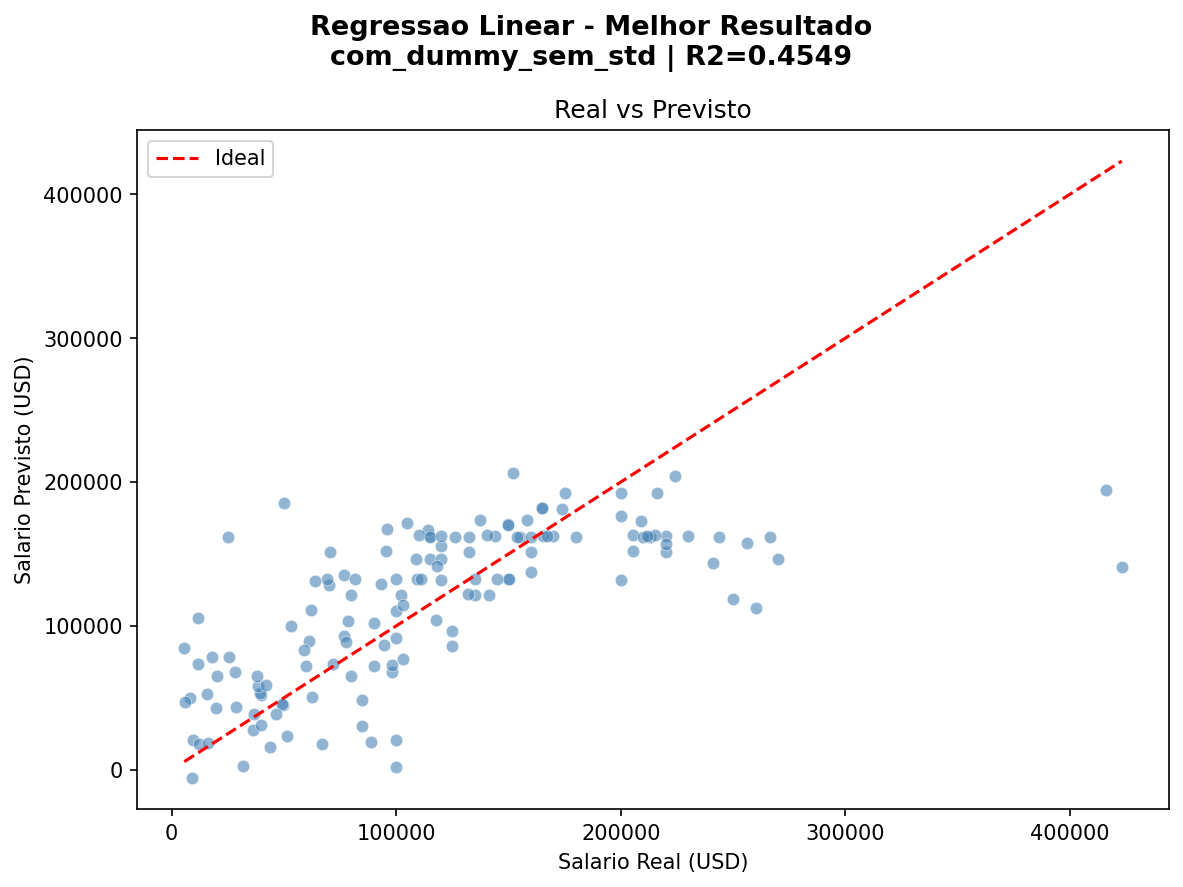
\includegraphics[width=0.8\textwidth]{imagens/regressao_linear/real_vs_previsto_lr.png}
    \caption{Valores reais vs.\ previstos --- Regressão Linear (base \textit{com\_dummy\_sem\_std})}
    \label{fig:lr_real_vs_previsto}
\end{figure}

Os resultados indicam que o One-Hot Encoding oferece ganho de $\sim$3 pontos percentuais de $R^2$ em relação ao Label Encoding, ao evitar relações ordinais artificiais entre categorias. A padronização não apresentou impacto significativo, o que é esperado, pois a Regressão Linear por mínimos quadrados ordinários não depende da escala dos atributos para a otimização.

O modelo explica aproximadamente 45\% da variância salarial, com erro médio de $\sim$\$40.000, indicando capacidade preditiva moderada.


\subsection{Regressão Polinomial}

Rever resultados da Regressão Polinomial.


\subsection{Árvore de Decisão}

Para a Árvore de Decisão, foram testadas profundidades máximas de 1 a 20 em todas as bases de pré-processamento, totalizando 80 experimentos. A Tabela~\ref{tab:dt_resultados} apresenta os melhores resultados por base.

\begin{table}[H]
\centering
\caption{Melhores resultados da Árvore de Decisão por base de pré-processamento}
\label{tab:dt_resultados}
\begin{tabular}{|l|c|c|c|c|c|}
\hline
\textbf{Base} & \textbf{Profundidade} & \textbf{$R^2$} & \textbf{MAE (USD)} & \textbf{RMSE (USD)} & \textbf{MAPE (\%)} \\ \hline
sem\_dummy\_com\_std & 3 & \textbf{0,5142} & \textbf{37.020} & \textbf{52.967} & \textbf{64,93} \\ \hline
com\_dummy\_com\_std & 3 & 0,5115 & 36.792 & 53.116 & 68,89 \\ \hline
sem\_dummy\_sem\_std & 3 & 0,5142 & 37.020 & 52.967 & 64,93 \\ \hline
com\_dummy\_sem\_std & 3 & 0,5115 & 36.792 & 53.116 & 68,89 \\ \hline
\end{tabular}
\end{table}

A melhor configuração utilizou profundidade 3 na base \textit{sem\_dummy\_com\_std}, obtendo o maior $R^2$ entre todos os modelos avaliados ($R^2 = 0{,}5142$) com $MAE \approx \$37.020$ e $RMSE \approx \$52.967$.

\begin{figure}[H]
    \centering
    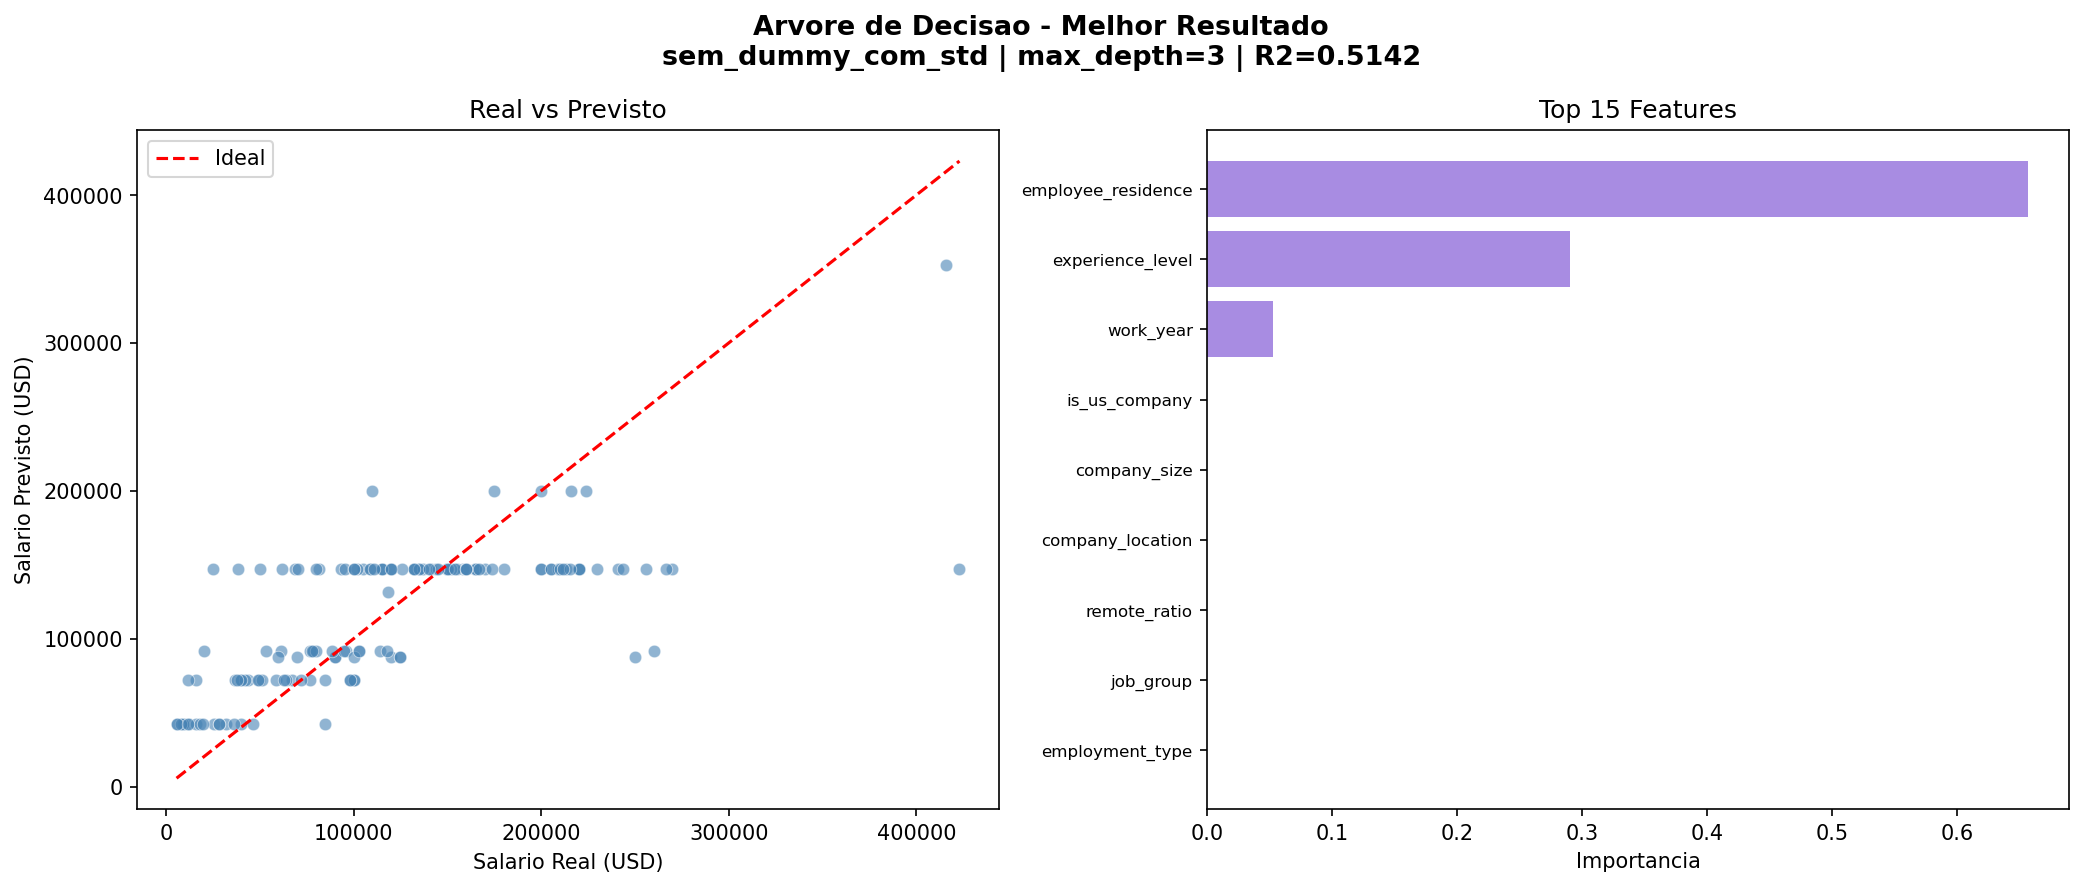
\includegraphics[width=1\textwidth]{imagens/arvore_decisao/real_vs_previsto_dt.png}
    \caption{Árvore de Decisão --- melhor resultado: valores reais vs.\ previstos e importância das features (profundidade 3)}
    \label{fig:dt_real_vs_previsto}
\end{figure}

Um resultado notável é que profundidades maiores que 3 degradaram o desempenho significativamente. Na base \textit{com\_dummy\_com\_std}, o $R^2$ caiu de 0,51 (profundidade 3) para 0,20 (profundidade 4) e chegou a valores negativos em profundidades acima de 6. Esse comportamento indica \textit{overfitting} severo quando a árvore cresce, causado pelo tamanho reduzido do dataset (565 amostras).

A padronização não alterou os resultados (como esperado, pois árvores de decisão são invariantes à escala). As bases com \textit{Label Encoding} e \textit{One-Hot Encoding} obtiveram desempenho semelhante na profundidade 3.


\subsection{Random Forest}

O Random Forest foi avaliado com um grid de hiperparâmetros: número de árvores $\in \{50, 100, 200\}$ e profundidade máxima $\in \{5, 10, 15, 20\}$, nas quatro bases, totalizando 48 experimentos. A Tabela~\ref{tab:rf_resultados} apresenta os melhores resultados por base.

\begin{table}[H]
\centering
\caption{Melhores resultados do Random Forest por base de pré-processamento}
\label{tab:rf_resultados}
\begin{tabular}{|l|l|c|c|c|}
\hline
\textbf{Base} & \textbf{Config.} & \textbf{$R^2$} & \textbf{MAE (USD)} & \textbf{RMSE (USD)} \\ \hline
com\_dummy\_sem\_std & 200 ár., prof.\ 10 & \textbf{0,4505} & \textbf{38.393} & \textbf{56.333} \\ \hline
com\_dummy\_com\_std & 50 ár., prof.\ 10 & 0,4495 & 38.410 & 56.382 \\ \hline
sem\_dummy\_com\_std & 50 ár., prof.\ 5 & 0,4393 & 38.915 & 56.903 \\ \hline
sem\_dummy\_sem\_std & 50 ár., prof.\ 5 & 0,4393 & 38.915 & 56.903 \\ \hline
\end{tabular}
\end{table}

A melhor configuração utilizou 200 árvores com profundidade 10 na base \textit{com\_dummy\_sem\_std}, obtendo $R^2 = 0{,}4505$.

\begin{figure}[H]
    \centering
    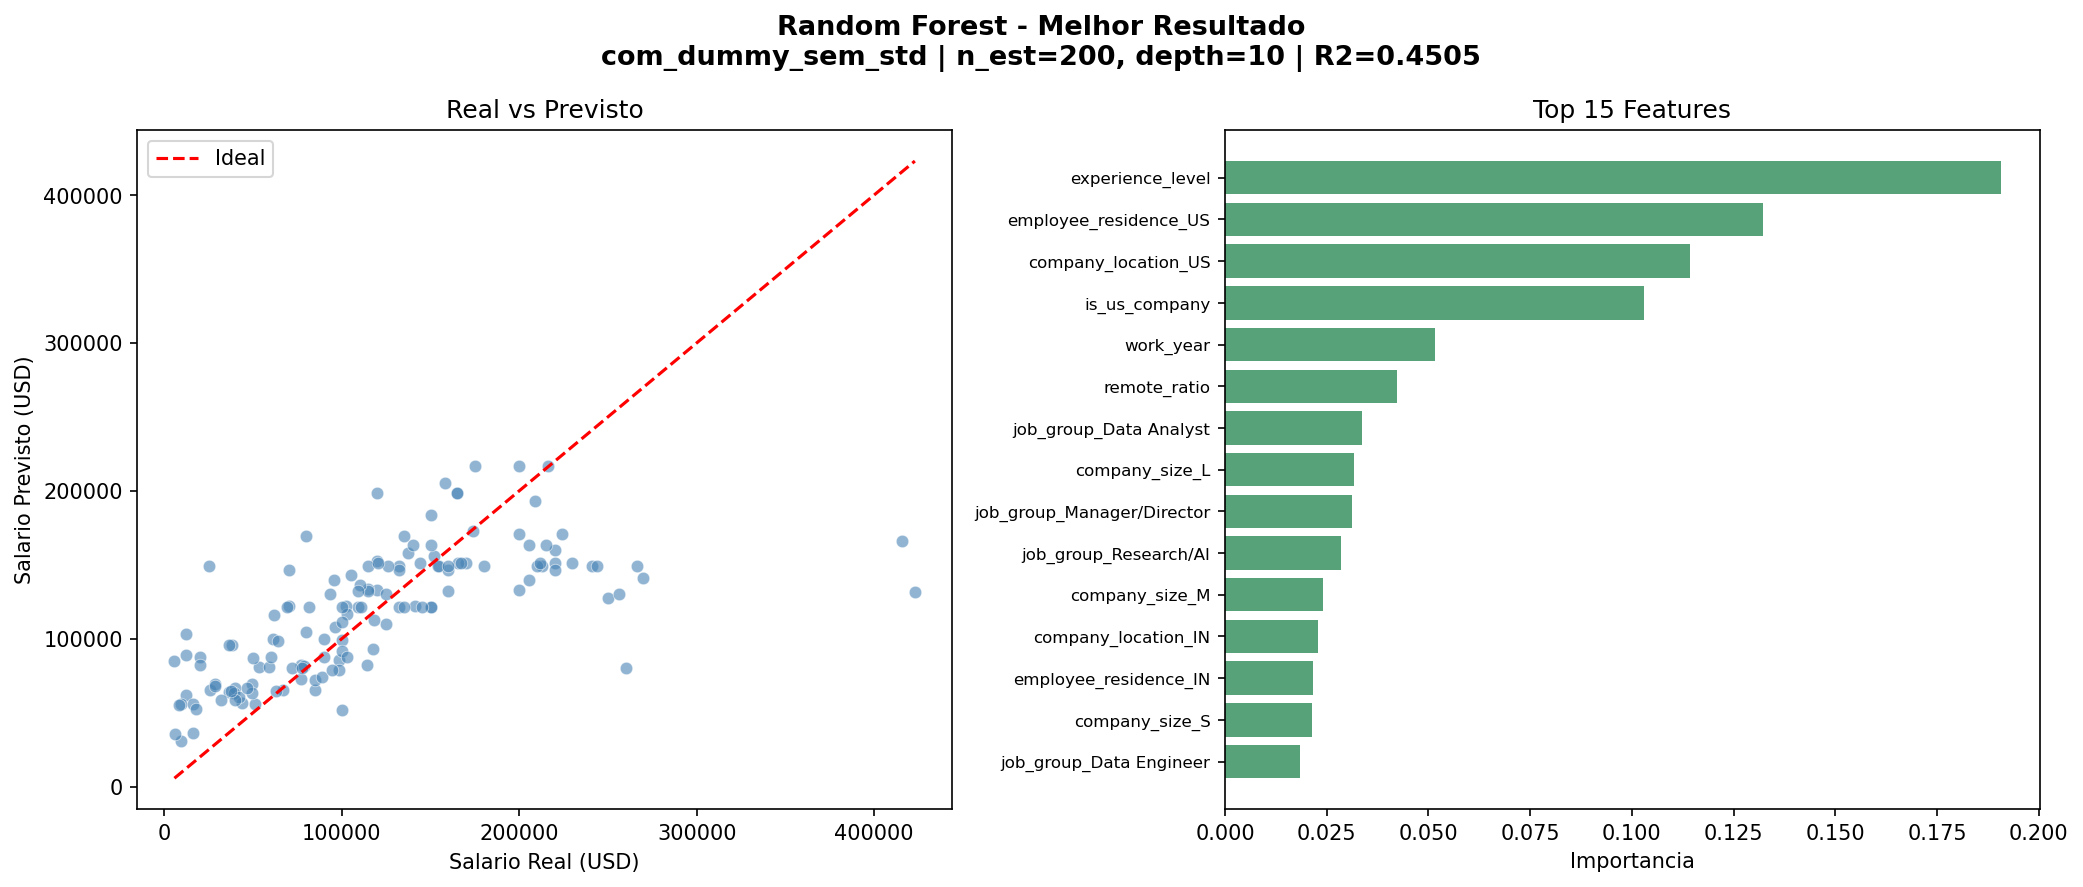
\includegraphics[width=1\textwidth]{imagens/random_forest/real_vs_previsto_rf.png}
    \caption{Random Forest --- melhor resultado: valores reais vs.\ previstos e importância das features}
    \label{fig:rf_real_vs_previsto}
\end{figure}

Um resultado surpreendente é que o Random Forest não superou a Árvore de Decisão simples nem a Regressão Linear. Isso pode ser explicado pelo tamanho reduzido do dataset: com apenas 565 amostras, o \textit{ensemble} não consegue explorar variabilidade suficiente entre as árvores. Além disso, a limitação de \texttt{max\_features=10} restringiu a quantidade de atributos disponíveis em cada divisão.

As bases com \textit{One-Hot Encoding} apresentaram desempenho ligeiramente superior ($R^2 \approx 0{,}45$) comparado ao \textit{Label Encoding} ($R^2 \approx 0{,}44$).


\subsection{Support Vector Machines (SVM)}

Para a aplicação do algoritmo de Support Vector Machines em regressão (SVR), foram avaliadas 6 configurações distintas de hiperparâmetros em cada uma das 4 bases de pré-processamento, totalizando 24 experimentos. Devido à alta sensibilidade do SVR à escala dos dados, tanto os atributos quanto a variável alvo (\textit{salary\_in\_usd}) foram padronizados internamente por meio de um \textit{Pipeline} com \textit{StandardScaler} e \textit{TransformedTargetRegressor}, garantindo que a escala salarial (de \$2K a \$600K) não prejudicasse o desempenho do modelo.

\subsubsection{Configurações Avaliadas}

Foram testados três tipos de kernel --- linear, RBF e polinomial (grau 2) --- com diferentes valores do parâmetro de regularização $C$ e margem de tolerância $\epsilon$. A Tabela~\ref{tab:svm_configs} resume as configurações avaliadas.

\begin{table}[H]
\centering
\caption{Configurações de hiperparâmetros avaliadas para o SVR}
\label{tab:svm_configs}
\begin{tabular}{|l|c|c|c|c|}
\hline
\textbf{Kernel} & \textbf{C} & \textbf{$\epsilon$} & \textbf{$\gamma$} & \textbf{Grau} \\ \hline
Linear & 1.0 & 0.1 & --- & --- \\ \hline
Linear & 10.0 & 0.1 & --- & --- \\ \hline
RBF & 10.0 & 0.1 & scale & --- \\ \hline
RBF & 100.0 & 0.1 & scale & --- \\ \hline
RBF & 100.0 & 0.2 & auto & --- \\ \hline
Polinomial & 10.0 & 0.1 & scale & 2 \\ \hline
\end{tabular}
\end{table}

\subsubsection{Resultados Obtidos}

A melhor configuração encontrada utilizou \textbf{kernel linear} com $C=1.0$ e $\epsilon=0.1$ na base \textit{com\_dummy\_com\_std} (codificação \textit{one-hot} com padronização), obtendo os seguintes resultados:

\begin{itemize}
    \item $R^2 = 0{,}4394$
    \item $MAE = 37.633{,}87$ USD
    \item $RMSE = 56.901{,}26$ USD
    \item $MAPE = 65{,}73\%$
\end{itemize}

A Tabela~\ref{tab:svm_resultados} apresenta os melhores resultados por tipo de kernel na base com melhor desempenho.

\begin{table}[H]
\centering
\caption{Melhores resultados do SVR por tipo de kernel (base \textit{com\_dummy\_com\_std})}
\label{tab:svm_resultados}
\begin{tabular}{|l|c|c|c|c|}
\hline
\textbf{Kernel} & \textbf{$R^2$} & \textbf{MAE (USD)} & \textbf{RMSE (USD)} & \textbf{MAPE (\%)} \\ \hline
Linear ($C=1.0$) & \textbf{0,4394} & \textbf{37.633} & \textbf{56.901} & \textbf{65,73} \\ \hline
RBF ($C=10.0$) & 0,3451 & 39.446 & 61.500 & 73,63 \\ \hline
Polinomial (grau 2) & 0,2366 & 44.082 & 66.397 & 92,04 \\ \hline
\end{tabular}
\end{table}

A Figura~\ref{fig:svm_real_vs_previsto} apresenta o gráfico de dispersão dos valores reais versus previstos para a melhor configuração.

\begin{figure}[H]
    \centering
    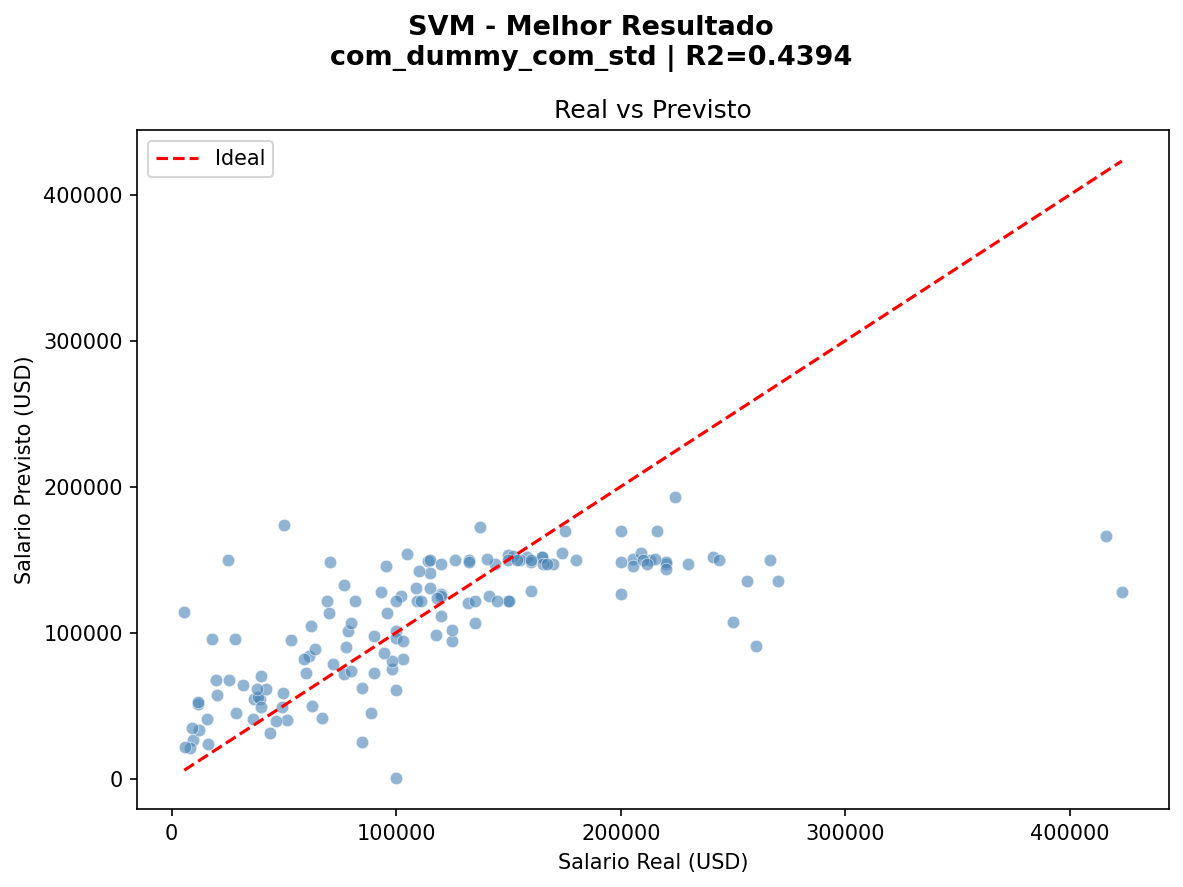
\includegraphics[width=0.8\textwidth]{imagens/svm/real_vs_previsto_svm.png}
    \caption{Valores reais vs.\ previstos --- melhor modelo SVR (kernel linear, $C=1.0$)}
    \label{fig:svm_real_vs_previsto}
\end{figure}

\subsubsection{Análise e Discussão}

Os resultados indicam que o kernel linear obteve o melhor desempenho entre as configurações testadas, sugerindo que as relações lineares presentes nos dados já são suficientes para a capacidade do SVR neste problema. Os kernels RBF e polinomial, apesar de permitirem modelar não linearidades, não apresentaram ganhos, possivelmente devido à alta dimensionalidade do espaço de atributos com \textit{one-hot encoding}.

Observa-se também que a padronização não alterou os resultados do kernel linear (bases \textit{com\_dummy\_com\_std} e \textit{com\_dummy\_sem\_std} apresentaram métricas idênticas), o que é esperado, pois o \textit{Pipeline} interno já aplica \textit{StandardScaler}.

Na base sem variáveis dummy (\textit{Label Encoding}), o desempenho do kernel linear foi ligeiramente inferior ($R^2 = 0{,}4139$), indicando que a codificação \textit{one-hot} favorece o SVR ao evitar relações ordinais artificiais entre as categorias.

Por outro lado, o kernel polinomial com \textit{Label Encoding} apresentou $R^2$ negativo ($-0{,}4615$), evidenciando que a combinação de codificação ordinal com transformações polinomiais gera artefatos que prejudicam significativamente o modelo.

O $R^2$ de 0,44 indica que o SVR explica menos da metade da variância dos salários, e o MAPE de 65,73\% reflete uma margem de erro elevada nas previsões individuais. Esses resultados colocam o SVR em uma posição intermediária entre os modelos avaliados.


\subsection{Redes Neurais (MLP)}

Para a aplicação de redes neurais na tarefa de regressão, foi utilizado o \textit{MLPRegressor} da biblioteca scikit-learn. Assim como no SVR, os atributos e a variável alvo foram padronizados internamente via \textit{Pipeline} com \textit{StandardScaler} e \textit{TransformedTargetRegressor}, uma vez que redes neurais são altamente sensíveis à escala dos dados e a variável \textit{salary\_in\_usd} possui amplitude elevada, o que pode causar instabilidade nos gradientes do otimizador Adam.

Foram avaliadas 6 configurações distintas de arquitetura em cada uma das 4 bases de pré-processamento, totalizando 24 experimentos.

\subsubsection{Configurações Avaliadas}

As arquiteturas testadas variaram em número de camadas ocultas (1 a 3), número de neurônios por camada, função de ativação (\textit{relu} e \textit{tanh}) e fator de regularização L2 ($\alpha$). Todos os modelos utilizaram o otimizador Adam com taxa de aprendizado adaptativa, \textit{early stopping} e \textit{random\_state} fixo para reprodutibilidade. A Tabela~\ref{tab:mlp_configs} resume as configurações avaliadas.

\begin{table}[H]
\centering
\caption{Configurações de arquitetura avaliadas para o MLPRegressor}
\label{tab:mlp_configs}
\begin{tabular}{|c|c|c|}
\hline
\textbf{Camadas ocultas} & \textbf{Ativação} & \textbf{$\alpha$} \\ \hline
(32,) & relu & 0,0001 \\ \hline
(64,) & relu & 0,0001 \\ \hline
(128, 64) & relu & 0,0001 \\ \hline
(64,) & tanh & 0,0001 \\ \hline
(128, 64) & tanh & 0,001 \\ \hline
(128, 64, 32) & relu & 0,001 \\ \hline
\end{tabular}
\end{table}

\subsubsection{Resultados Obtidos}

A melhor configuração encontrada utilizou a arquitetura \textbf{(128, 64)} com função de ativação \textbf{tanh} e $\alpha = 0{,}001$ na base \textit{sem\_dummy\_com\_std} (codificação \textit{Label Encoding} com padronização), obtendo os seguintes resultados:

\begin{itemize}
    \item $R^2 = 0{,}4291$
    \item $MAE = 37.982{,}44$ USD
    \item $RMSE = 57.419{,}84$ USD
    \item $MAPE = 78{,}06\%$
\end{itemize}

A Tabela~\ref{tab:mlp_resultados} apresenta os melhores resultados por base de pré-processamento.

\begin{table}[H]
\centering
\caption{Melhor resultado do MLPRegressor por base de pré-processamento}
\label{tab:mlp_resultados}
\begin{tabular}{|l|l|c|c|c|}
\hline
\textbf{Base} & \textbf{Arquitetura} & \textbf{$R^2$} & \textbf{MAE (USD)} & \textbf{RMSE (USD)} \\ \hline
sem\_dummy\_com\_std & (128, 64) tanh & \textbf{0,4291} & \textbf{37.982} & \textbf{57.419} \\ \hline
com\_dummy\_com\_std & (128, 64) tanh & 0,4116 & 38.988 & 58.293 \\ \hline
sem\_dummy\_sem\_std & (128, 64) tanh & 0,4291 & 37.982 & 57.419 \\ \hline
com\_dummy\_sem\_std & (128, 64) tanh & 0,4116 & 38.988 & 58.293 \\ \hline
\end{tabular}
\end{table}

A Figura~\ref{fig:nn_real_vs_previsto} apresenta o gráfico de dispersão dos valores reais versus previstos para a melhor configuração.

\begin{figure}[H]
\centering
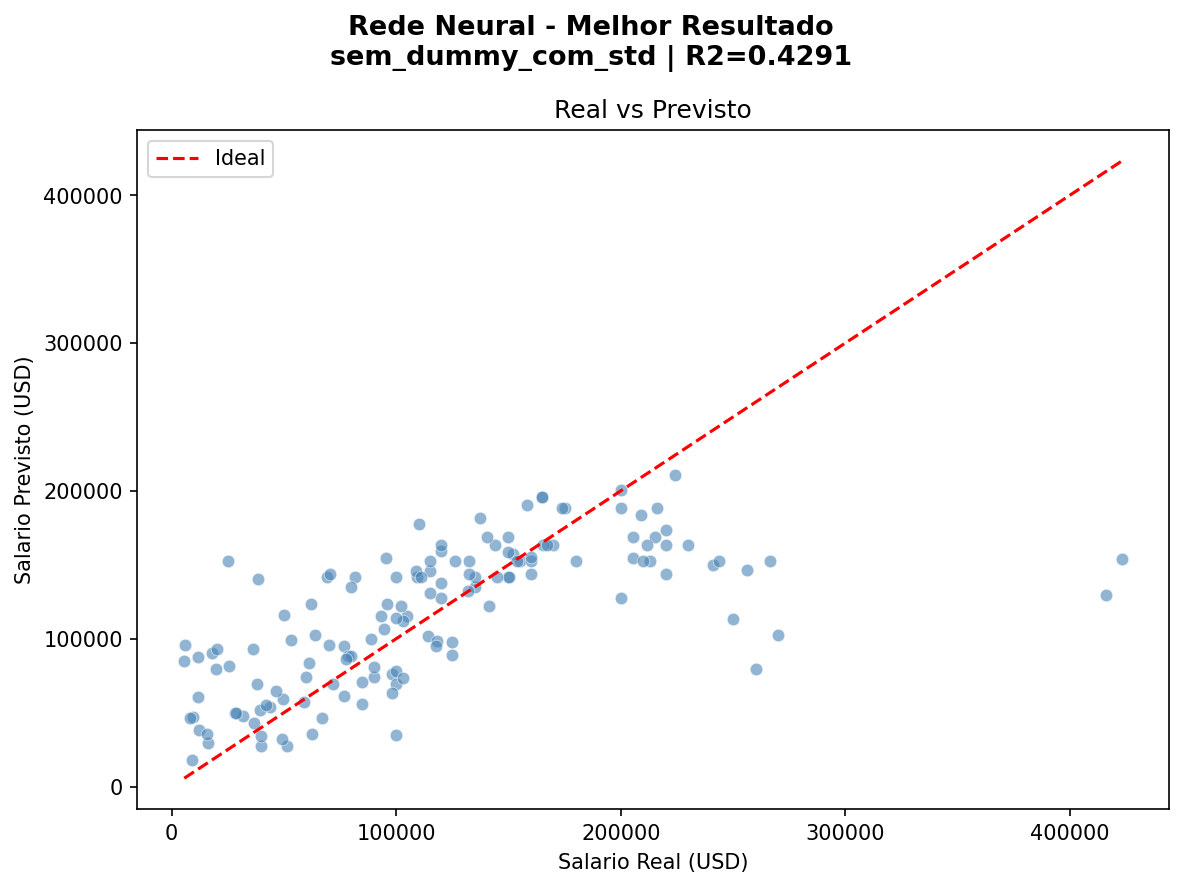
\includegraphics[width=0.8\linewidth]{imagens/redes_neurais/real_vs_previsto_nn.png}
\caption{Valores reais vs.\ previstos --- melhor modelo MLP (128, 64), tanh, $\alpha=0{,}001$}
\label{fig:nn_real_vs_previsto}
\end{figure}

\subsubsection{Análise e Discussão}

Os resultados revelam que a função de ativação \textit{tanh} superou consistentemente a \textit{relu} nas configurações de duas camadas, sugerindo que a simetria da função tangente hiperbólica ao redor de zero é benéfica para este problema. A regularização com $\alpha = 0{,}001$ também se mostrou importante para controlar o \textit{overfitting}, especialmente nas arquiteturas mais profundas.

Um resultado notável é que a arquitetura mais simples, com apenas 32 neurônios em uma camada, apresentou $R^2$ negativo ($-0{,}7196$) na base com \textit{one-hot encoding}, indicando que a rede não teve capacidade suficiente para aprender os padrões nessa dimensionalidade elevada. Em contrapartida, a mesma arquitetura com \textit{Label Encoding} obteve $R^2 = 0{,}3656$, demonstrando que a dimensionalidade reduzida facilita o aprendizado em redes menores.

Assim como observado no SVR, a padronização externa não alterou os resultados, já que o \textit{Pipeline} interno aplica \textit{StandardScaler} automaticamente. As bases com e sem padronização externa apresentaram métricas idênticas para cada codificação.

O melhor $R^2$ obtido (0,4291) indica que o MLPRegressor explica aproximadamente 43\% da variância salarial, com um erro médio absoluto de cerca de \$38.000. Embora o desempenho seja competitivo com o SVR, o MAPE mais elevado (78\%) sugere maior dificuldade nas previsões percentuais, especialmente para salários mais baixos.


\subsection{Análise Comparativa}

A Tabela~\ref{tab:comparacao_final} consolida os melhores resultados de cada modelo.

\begin{table}[H]
\centering
\caption{Comparação dos melhores resultados por modelo}
\label{tab:comparacao_final}
\begin{tabular}{|l|l|c|c|c|c|}
\hline
\textbf{Modelo} & \textbf{Melhor base} & \textbf{$R^2$} & \textbf{MAE} & \textbf{RMSE} & \textbf{MAPE} \\ \hline
Árvore de Decisão & sem\_dummy\_com\_std & \textbf{0,514} & \textbf{37.020} & \textbf{52.967} & \textbf{64,9\%} \\ \hline
Regressão Linear & com\_dummy\_sem\_std & 0,455 & 39.763 & 56.109 & 72,4\% \\ \hline
Random Forest & com\_dummy\_sem\_std & 0,450 & 38.393 & 56.333 & 77,1\% \\ \hline
SVM (linear) & com\_dummy\_com\_std & 0,439 & 37.633 & 56.901 & 65,7\% \\ \hline
Rede Neural & sem\_dummy\_com\_std & 0,429 & 37.982 & 57.419 & 78,1\% \\ \hline
\end{tabular}
\end{table}

A análise comparativa permite destacar os seguintes pontos:

\begin{enumerate}
    \item \textbf{A Árvore de Decisão obteve o melhor desempenho}, com $R^2 = 0{,}514$ e o menor RMSE (\$52.967). Sua profundidade 3, apesar de simples, capturou as divisões mais informativas do dataset. Esse resultado sugere que a relação entre os atributos e o salário pode ser representada por poucas regras bem definidas.

    \item \textbf{Modelos lineares apresentaram desempenho competitivo.} A Regressão Linear ($R^2 = 0{,}455$) e o SVR com kernel linear ($R^2 = 0{,}439$) obtiveram resultados próximos, indicando que componentes lineares explicam parte significativa da variância salarial.

    \item \textbf{Modelos mais complexos não superaram os mais simples.} O Random Forest, o SVR e a Rede Neural não ultrapassaram a Árvore de Decisão simples. Esse resultado é atribuído ao tamanho reduzido do dataset (565 amostras), que limita a capacidade de generalização dos modelos de maior capacidade.

    \item \textbf{O MAPE elevado em todos os modelos} (mínimo de 64,9\%) indica que a predição percentual é imprecisa, especialmente para salários mais baixos, onde erros absolutos representam uma fração maior do valor real.
\end{enumerate}


\section{Conclusão}

Este trabalho aplicou seis técnicas de aprendizado de máquina supervisionado para a predição salarial de profissionais de Ciência de Dados, utilizando o dataset ``Data Science Job Salaries''. Foram avaliadas diferentes configurações de pré-processamento, codificação de variáveis categóricas e hiperparâmetros, totalizando mais de 200 experimentos.

O modelo de Árvore de Decisão com profundidade 3 obteve o melhor desempenho ($R^2 = 0{,}514$), seguido pela Regressão Linear ($R^2 = 0{,}455$) e pelo Random Forest ($R^2 = 0{,}450$). Modelos mais complexos, como SVM e Redes Neurais, não apresentaram ganhos significativos em relação aos modelos mais simples.

Esses resultados indicam que, para datasets de tamanho reduzido (565 amostras), modelos mais simples tendem a generalizar melhor, evitando o \textit{overfitting} que afeta modelos de maior capacidade. A engenharia de atributos --- especialmente o agrupamento de cargos (\textit{job\_group}) e a identificação de empresas americanas (\textit{is\_us\_company}) --- demonstrou ser mais determinante para o desempenho do que a escolha do algoritmo em si.

O erro médio absoluto em torno de \$37.000--\$40.000 em todos os melhores modelos sugere que fatores relevantes para a determinação salarial não estão presentes no dataset, como anos de experiência específicos, habilidades técnicas, certificações e negociação individual. Futuras melhorias poderiam incluir o uso de datasets mais completos e de maior volume, técnicas de validação cruzada, e métodos de \textit{ensemble} mais sofisticados.


\bibliography{sbc-template.bib}
\end{document}
